%!TEX root =  ./JanasJanssenCuffaro-August2019.tex

%SUBSECTION 3.1
%\subsection{The quantum correlations} \label{2.1}

%SUBSUBSECTION 3.1.1
\subsubsection{Quantum formalism for one spin-$s$ particle} \label{2.1.1}

We review the formalism for spin angular momentum of particles of arbitrary integer or half-integer spin $s$, starting with the one-particle case.\footnote{Our presentation roughly follows the treatment of angular momentum in \citet[Vol.\ 2, Appendix C]{Messiah 1962}.} The state of a spin-$s$ particle with component $m\hbar$ in the $z$-direction is represented by a state vector $|s,m\rangle_z$ in a one-particle Hilbert space (where $\hbar \equiv h/2\pi$ and $h$ is Planck's constant). These vectors are simultaneous eigenvectors of the Hermitian operators 
\begin{equation}
\hat{S}_z, \quad \hat{S}^2\equiv \hat{S}_x^2+\hat{S}_y^2+\hat{S}_z^2,
\label{Sz and S^2}
\end{equation}
with eigenvalues $m \hbar$ (with $m \in \{ -s, \ldots, s\}$) and $s(s+1) \hbar^2$, respectively:
%\footnote{For the counterpart of Planck's constant in Bananaworld, see the paragraph following Eq.\ (\ref{cov def}).}
\begin{equation} 
\hat{S}_z |s,m\rangle_z =  m  \hbar \, |s,m\rangle_z,\quad \hat{S}^2 |s,m\rangle_z= s(s+1)   \hbar^2 \, |s,m\rangle_z,
\label{state dfn}
\end{equation} 
We will follow the common practice of setting $\hbar =1$. The operators $\hat{S}_x$, $\hat{S}_y$ and $\hat{S}_z$ can be thought of as components of a vector
\begin{equation}
\hat{\vec{S}} \equiv \left(\hat{S}_x, \hat{S}_y, \hat{S}_z \right).
\label{def S vector}
\end{equation}
The operator $\hat{S}^2$ represents the length of this vector. 

The simultaneous eigenvectors of $\hat{S}_z$ and $ \hat{S}^2$ form an orthonormal basis of the $(2s+1)$-dimensional one-particle Hilbert space,
\begin{equation}
\big\{|s,m \rangle_{z}\big\}_{m=-s}^s \;\; \mathrm{with} \;\; {_{z\!}}\langle s,  m | s,  m' \rangle_z = \delta_{mm'},
\label{onb one-particle Hilbert space}
\end{equation}
where $\delta_{mm'}$ is the Kronecker delta ($\delta_{mm'} = 1$ if $m=m'$ and $\delta_{mm'} = 0$ if $m \neq m'$). The operators $\hat{S}_x$, $\hat{S}_y$ and $\hat{S}_z$ satisfy the commutation relations 
\begin{equation}
[\hat{S}_x,\hat{S}_y]=i \hat{S}_z,\quad [\hat{S}_y,\hat{S}_z]=i \hat{S}_x,\quad [\hat{S}_z,\hat{S}_x]=i \hat{S}_y.
\label{ops dfn}
\end{equation}

We will also use the raising/lowering operators $\hat{S}_{\pm} \equiv \hat{S}_x\pm i \hat{S}_y$. The action of $\hat{S}_{\pm}$ on one of the orthonormal basis vectors $|s,m\rangle_z$ is given by
\begin{equation}
\hat{S}_\pm |s,m\rangle_z = C_\pm(s,m)|s,m \pm1\rangle_z.
\label{raising operator}
\end{equation}
Using that $|s,m\rangle_z$ and $|s,m\pm1\rangle_z$ are unit vectors, we can find expression for the constants $C_\pm(s,m)$. We do this for $C_+$. We start from
\begin{equation}
C_+(s,m)^2 = C_+(s,m)^2 {_z}\langle s,m+1|s,m+1\rangle_z = {_z\!}\langle s,m|\hat{S}_+^\dagger \hat{S}_+|s,m\rangle_{\!z}.
\label{raising norm 1}
\end{equation}
Since
\begin{equation}
\hat{S}_+^\dagger \hat{S}_+ = (\hat{S}_x-i \hat{S}_y)(\hat{S}_x+i \hat{S}_y) = \hat{S}_x^2+\hat{S}_y^2 +i[\hat{S}_x,\hat{S}_y]=\hat{S}^2 - \hat{S}_z^2-\hat{S}_z,
\label{raising}
\end{equation}
we can rewrite the right-hand side as
\begin{equation}
{_z\!}\langle s,m|\big(\hat{S}^2-\hat{S}_z^2-\hat{S}_z\big)|s,m\rangle_{\!z} = (s(s+1)-m(m+1)) \, {_z\!}\langle s,m|s,m\rangle_{\!z}.
\label{raising norm 2}
\end{equation}
Choosing $C_+(s,m)$ to be positive and real (the so-called Condon-Shortley convention), we conclude that
\begin{equation}
C_+(s,m)=\sqrt{s(s+1)-m(m+1)}.
\label{coef raising}
\end{equation}
A corollary of this phase convention is that the operator $i\hat{S}_y = \frac12 \hat{S}_{+}-\frac12 \hat{S}_-$ has real matrix elements in the $|s,m\rangle_{\!z}$ basis.

\begin{figure}[ht]
 \centering
   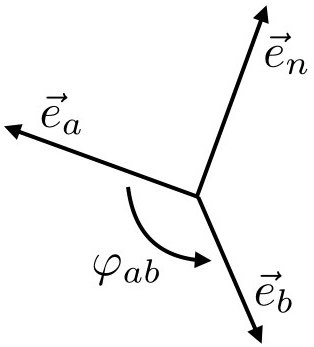
\includegraphics[width=1.4in]{rotation.jpeg} 
   \caption{Rotation by an angle $\varphi_{ab}$ about the direction $\vec{e}_n$, mapping $\vec{e}_z$ to $\vec{e}_a$.}
   \label{rotation}
\end{figure}


As we already saw in Section \ref{1.6}, one can also define spin operators associated with directions other than the Cartesian axes. The spin operator associated with the direction given by the unit vector $\vec{e}_a=(a_x,a_y,a_z)$ is defined as
\begin{equation}
\hat{S}_a \equiv \hat{\vec{S}} \cdot \vec{e}_a = \hat{S}_x a_x+\hat{S}_y a_y+\hat{S}_z a_z.
\label{spin op}
\end{equation}

Such spin operators generate rotations in Hilbert space. Let $\hat{S}_a$ and $\hat{S}_b$ be spin operators associated with the directions given by the unit vectors $\vec{e}_a$ and $\vec{e}_b$.  Let $\vec{e}_n$ be a unit vector in the direction of the cross product $\vec{e}_a\times \vec{e}_b$, so that we get from $\vec{e}_a$ to $\vec{e}_b$ by rotating around $\vec{e}_n$ by the angle $\varphi_{ab}$ between them (see Figure \ref{rotation}). This rotation is implemented in Hilbert space by the rotation operator $e^{-i \varphi_{ab} \hat{S}_n}$. It can be shown that the transformation from the spin operator $\hat{S}_a$ associated with $\vec{e}_a$ to the spin operator $\hat{S}_b$ associated with $\vec{e}_b$ is given by:
\begin{equation}
 \hat{S}_b = e^{-i\varphi_{ab} \hat{S}_n}\hat{S}_a e^{i\varphi_{ab}  \hat{S}_n}
\label{ops rot}
\end{equation}
\citep[Vol.\ 2, pp.\ 530--533; see also Baym 1969, pp.\ 305--307]{Messiah 1962}. The transformation of the eigenvectors of $\hat{S}_a$ to the eigenvectors of $\hat{S}_b$ is accordingly given by:\footnote{Whereas it takes some effort to prove the transformation law in Eq.\ (\ref{ops rot}), it is easy to see that this transformation law for operators entails the one for state vectors in Eq.\ (\ref{state rot}). Using Eq.\ (\ref{ops rot}), we can show that, whenever $|s, m\rangle_a$ is an eigenvector of $\hat{S}_a$ with eigenvalue $m$, $|s, m\rangle_b$ in Eq.\ (\ref{state rot}) is, in fact, an eigenvector of $\hat{S}_b$ with that same eigenvalue, as the notation suggests:
\begin{eqnarray*}
\hat{S}_b |s, m\rangle_b & \!\!\! = \!\!\! & \left( e^{-i\varphi_{ab} \hat{S}_n}\hat{S}_a e^{i\varphi_{ab}  \hat{S}_n} \right) \left( e^{-i \varphi_{ab} \hat{S}_n}|s,m\rangle_a\right) \\[.3 cm]
 & \!\!\! = \!\!\! & e^{-i\varphi_{ab} \hat{S}_n}\hat{S}_a |s,m\rangle_a = e^{-i\varphi_{ab} \hat{S}_n} m |s,m\rangle_a = m |s,m\rangle_b.
\end{eqnarray*}}
\begin{equation}
|s,m\rangle_b = e^{-i \varphi_{ab} \hat{S}_n}|s,m\rangle_a.
\label{state rot}
\end{equation}

We now show that, in the special case that $s = \sfrac12$ and $\vec{e}_a$ to $\vec{e}_b$ are in the $xz$-plane, the transformation law in Eq.\ (\ref{state rot}) reduces to the one in Eq.\ (\ref{QM2}) in Section \ref{1.5}. For $s = \sfrac12$, the elements of the matrices representing the spin operators $\hat{S}_x$, $\hat{S}_y$ and $\hat{S}_z$  in the orthonormal basis  in Eq.\ (\ref{onb one-particle Hilbert space}) of eigenvectors of $\hat{S}_z$ are $\sfrac12$ times the Pauli matrices (as long as the Condon-Shortley convention mentioned above is adopted):
\begin{equation}
\begin{array}{c}
\hat{S}_x = \sfrac12 \, \hat{\sigma}_x = \frac12 \begin{pmatrix} 
0  \! & \! 1 \\
1 \! & \! 0
\end{pmatrix},  \\[.5cm]
\hat{S}_y = \sfrac12 \, \hat{\sigma}_y = \frac12 \begin{pmatrix} 
0  \! & \! - i \\
i \! & \! 0
\end{pmatrix}, \\[.5cm]
\hat{S}_z = \sfrac12 \, \hat{\sigma}_z = \frac12 \begin{pmatrix} 
1 \! & \! 0 \\
0 \! & \! -1
\end{pmatrix}.
\end{array}
\label{Pauli matrices}
\end{equation}
One readily verifies that these matrices satisfy the commutation relations in Eq.\ (\ref{ops dfn}).

For $s = \sfrac12$, the rotation operator $e^{-i\vartheta \hat{S}_n}$ has a particularly simple form, which we can find using 
%\citep[pp.\ 306--307]{Baym 1969}. 
the completeness of the orthonormal basis of eigenvectors 
\begin{equation}
%\big\{| {\textstyle \frac12,\frac12} \rangle_{n}, | {\textstyle \frac12, -\frac12} \rangle_{n} \big\}
\left\{ \left|  \sfrac12,\sfrac12 \right\rangle_{n}, \left|  \sfrac12, -\sfrac12 \right\rangle_{n} \right\}
\label{onb spin S_n}
\end{equation}
of the spin operator $\hat{S}_n$ associated with the unit vector $\vec{e}_n$. For the purposes of this calculation, we revert to the notation $| \pm \rangle_n$ of Section \ref{1.5} for these eigenvectors. With the help of the resolution of unity in the basis of these eigenvectors,
\begin{equation}
\hat{1} = |+\rangle_{\!n} \, _{n\!}\langle +| \; + \; |-\rangle_{\!n} \, _{n\!}\langle -|
\label{rot proof 1}
\end{equation}
we can write the spectral decomposition of the spin operator $\hat{S}_n$ as
\begin{equation}
\hat{S}_n = \textstyle{\frac12} |+\rangle_{\!n} \, _{n\!}\langle + | \, - \, \textstyle{\frac12} |-\rangle_{\!n} \, _{n\!}\langle -|,
\label{rot proof 2}
\end{equation}
and the spectral decomposition of the rotation operator $e^{-i\vartheta \hat{S}_n}$ as
\begin{equation}
e^{-i\vartheta \hat{S}_n} = e^{-i\vartheta/2} |+\rangle_{\!n} \, _{n\!}\langle + | \; + \; e^{i\vartheta/2} |-\rangle_{\!n} \, _{n\!}\langle -|.
\label{rot proof 3}
\end{equation}
Collecting terms with cosines and sines and using Eqs.\ (\ref{rot proof 1})--(\ref{rot proof 2}), we find that
\begin{eqnarray}
e^{-i\vartheta \hat{S}_n} & \!\! = \!\! & \Big( \cos{\!(\vartheta/2)} - i \, \sin{\!(\vartheta/2)} \Big) |+\rangle_{\!n} \, _{n\!}\langle + | \nonumber \\
 & & \quad \quad \quad \quad + \; \Big(\cos{\!(\vartheta/2)} + i \, \sin{\!(\vartheta/2)} \Big) | -\rangle_{\!n} \, _{n\!}\langle - | \nonumber \\
 & \!\! = \!\!  & \cos{\!(\vartheta/2)} \, \hat{1} - i \sin{\!(\vartheta/2)} \, 2\hat{S}_n
 \label{rot proof 4}
\end{eqnarray}
Note that we got from the angle $\vartheta$ to the half-angle $\vartheta/2$ because of the factor of $\sfrac12$ in the eigenvalues $\hbar/2$ of the spin operator $\hat{S}_n$. 

To recover Eq.\ (\ref{QM2}), we choose $\vec{e}_n$ in the $y$-direction and $\vec{e}_a$ in the $z$-direction. Hence, $\hat{S}_n = \hat{S}_y$ and $\hat{S}_z = \hat{S}_a$. In that case, as we saw in Eq.\ (\ref{Pauli matrices}), the matrix representing $2\hat{S}_y$  in the basis $\big\{| + \rangle_{a}, | - \rangle_{a} \big\}$ is the Pauli matrix $\hat{\sigma}_y$. The matrix elements representing the rotation operator $e^{-i\vartheta \hat{S}_n}$ in this basis is then given by:
\begin{equation}
\cos{\! \left(\frac\vartheta2\right)}  
\begin{pmatrix} 
1  \! & \! 0 \\[.2 cm]
0 \! & \! 1
\end{pmatrix} 
\, - \, i \sin{\! \left(\frac\vartheta2\right)} 
\begin{pmatrix} 
0  \! & \! - i \\[.2 cm]
i \! & \! 0
\end{pmatrix}
= 
\begin{pmatrix} 
\cos{\!(\vartheta/2)} \! & \! - \sin{\!(\vartheta/2)} \\[.2 cm]
\sin{\!(\vartheta/2)} \! & \! \cos{\!(\vartheta/2)}
\end{pmatrix}.
\label{spin 1/2 rotation}
\end{equation}
From this matrix we can read off the components of the eigenvectors of $\hat{S}_b$ associated with a unit vector $\vec{e}_b$ in the $xz$-plane obtained by rotating the eigenvectors of $\hat{S}_a$ associated with a unit vector $\vec{e}_a = \vec{e}_z$ (cf.\ Eq.\ (\ref{state rot})):
\begin{equation}
| \pm \rangle_b = e^{-i \varphi_{ab} \hat{S}_y} | \pm \rangle_a.
\end{equation}
Using the resolution of unity in the $\{| \pm \rangle_a \}$ basis, we find:
\begin{eqnarray}
| \pm \rangle_b & \!\!\! =  \!\!\! & \Big( |+\rangle_{\!a} \, _{a\!}\langle +| \; + \; |-\rangle_{\!a} \, _{a\!}\langle -| \Big) e^{-i \varphi_{ab} \hat{S}_y} | \pm \rangle_a
\nonumber \\
 & \!\!\! =  \!\!\! & \Big(\!\,  _{a\!}\langle +| e^{-i \varphi_{ab} \hat{S}_y} | \pm \rangle_a \! \Big) |+\rangle_a 
 \; + \; \Big(\!\,  _{a\!}\langle -| e^{-i \varphi_{ab} \hat{S}_y} | \pm \rangle_a \! \Big) |-\rangle_a 
\label{b +/- trans law}
\end{eqnarray}
Using Eq.\ (\ref{spin 1/2 rotation}) with $\vartheta = \varphi_{ab}$ for the matrix elements of the rotation operator in the $\{ | \pm \rangle_a \}$ basis,
\begin{equation}
_{a\!}\langle \pm | e^{-i \varphi_{ab} \hat{S}_y} | \pm \rangle_a 
=
\begin{pmatrix} 
\cos(\varphi_{ab}/2) \! & \! -\sin(\varphi_{ab}/2)\\[.3 cm]
\sin(\varphi_{ab}/2) \! & \! \cos(\varphi_{ab}/2)
\end{pmatrix},
\label{spin 1/2 rotation 2}
\end{equation}
we arrive at  
\begin{eqnarray}
|+\rangle_b &\!\!=\!\!& \cos\left(\frac{\varphi_{ab}}{2}\right)|+\rangle_a+\sin\left(\frac{\varphi_{ab}}{2}\right)|-\rangle_a, \nonumber \\[.3 cm]
|-\rangle_b &\!\!=\!\!& - \sin\left(\frac{\varphi_{ab}}{2}\right)|+\rangle_a+\cos\left(\frac{\varphi_{ab}}{2}\right)|-\rangle_a.
\label{b +/- trans law 2}
\end{eqnarray}
This is just the inverse of the transformation from $|\pm \rangle_b$ to $|\pm\rangle_a$ in Eq. (\ref{QM2}). We used Eq.\ (\ref{QM2}) to show that the singlet state for a pair of spin-$\frac12$ particles has the same form in orthonormal bases $\{ | \pm \rangle_a \}$ and $\{ | \pm \rangle_b \}$ (see Eqs.\ (\ref{singlet state s=1/2 simple})--(\ref{QM3})). We concluded that this singlet state has the same form in \emph{any} orthonormal basis  $\{ | \pm \rangle_n \}$. Strictly speaking, our derivation of Eq.\ (\ref{b +/- trans law 2}) only allows us to claim this for orthonormal bases of eigenvectors of spin operators associated with unit vectors in the $xz$-plane. However, since for any two unit vectors $\vec{e}_a$ and $\vec{e}_b$, we can choose the plane spanned by those two vectors to be the $xz$ plane, this result holds for \emph{any} orthonormal basis  $\{ | \pm \rangle_n \}$.

We now turn to the special case $s=0$. Eq.\ (\ref{state dfn}) tells us that $\hat{S}^2 |0,m\rangle_z=0$. Using that $\hat{S}^2 = \hat{S}_y^2 + \hat{S}_x^2 +\hat{S}_z^2$, we thus have
\begin{eqnarray}
0 &\!\!=\!\!& {_z} \langle 0,m|\hat{S}_x^2 |0,m\rangle_z + {_z}\langle 0,m|\hat{S}_y^2 |0,m\rangle_z + {_z}\langle 0,m|\hat{S}_z^2 |0,m\rangle{_z} \nonumber \\[.3 cm]
&\!\!=\!\!& \Big|\hat{S}_x|0,m\rangle_z \Big|^2 + \Big|\hat{S}_y|0,m\rangle_z \Big|^2 +\Big|\hat{S}_z|0,m\rangle_z \Big|^2.
\label{zero spin}
\end{eqnarray}
This last expression, being a sum of squared absolute values, can only vanish if 
\begin{equation}
\hat{S}_x |0,m\rangle_z = \hat{S}_y |0,m\rangle_z = \hat{S}_z |0,m\rangle_z = 0. 
\label{zero comps}
\end{equation}
This enforces that $m=0$ (see Eq.\ (\ref{ops dfn})). More generally, it means that the singlet state has zero spin angular momentum along any direction. Hence we must have $\hat{S}_n|0,0\rangle_z = 0$. This implies that the singlet state is invariant under rotation through an angle $\vartheta$ with respect to any direction $\vec{e}_n$:
\begin{equation}
e^{-i\vartheta \hat{S}_n }|0,0\rangle_{z} = \sum_{k=0}^\infty \frac{(-i\vartheta)^k}{k!}\hat{S}^k_n|0,0\rangle_z = |0,0\rangle_z,
\label{singlet rot}
\end{equation}
as the only contribution to the sum comes from the $k=0$ term.

%SUBSUBSECTION 3.1.2
\subsubsection{Quantum formalism for two spin-$s$ particles in the singlet state} \label{2.1.2}

In Section \ref{1.5}, we considered the singlet state for a pair of spin-$\frac12$ particles (see Eq.\ (\ref{singlet state s=1/2 simple})). For the rest of this section, we consider the singlet state for two particles of any (half-)integer spin $s$. Alice performs measurements on particle 1, with a one-particle Hilbert space spanned by $\{|s,m_1\rangle_{1z}\}_{m_1=-s}^s$ and one-particle spin operators $\hat{S}_{1x},\hat{S}_{1y},\hat{S}_{1z}$. Similarly, Bob performs measurements on particle 2, with a one-particle Hilbert space spanned by $\{|s,m_2\rangle_{2z}\}_{m_2=-s}^s$ and one-particle spin operators $\hat{S}_{2x}$, $\hat{S}_{2y}$ and $\hat{S}_{2z}$. The two-particle Hilbert space therefore has dimension $(2s+1)^2$ and is spanned by the orthonormal basis
\begin{equation}
\big\{|s,m_1\rangle_{1z} \, |s,m_2\rangle_{2z}\big\}_{m_1, m_2=-s}^s.
\label{2 particle basis}
\end{equation}
The spin operators on this two-particle Hilbert space are 
\begin{equation}
\hat{S}_{n}=\hat{S}_{1n}+\hat{S}_{2n}.
\label{total spin ops}
\end{equation}
%(see Eq.\ (\ref{spin op}) for the definition of $\hat{S}_n$ in the one-particle case). 
The action of these operators on the basis vectors in Eq.\ (\ref{2 particle basis}) is given by:
\begin{equation}
\hat{S}_{n} \, |s,m_1\rangle_{1z} \, |s,m_2\rangle_{2z} = \Big( \hat{S}_{1n} \, |s,m_1\rangle_{1z} \Big) |s,m_2\rangle_{2z}
+ |s,m_1\rangle_{1z} \Big( \hat{S}_{2n} |s,m_2\rangle_{2z} \Big).
\label{total spin ops action}
\end{equation}

We now show that the two-particle state 
\begin{equation}
|0,0\rangle_{\!12} = \sum_{m=-s}^s \frac{(-1)^{s-m}}{\sqrt{2s+1}} |s,m\rangle_{1z}|s,-m\rangle_{2z}
\label{singlet state}
\end{equation}
is the singlet state of two particles of any (half-)integer spin $s$.\footnote{For $s=0$, Eq.\ (\ref{singlet state}) trivially reduces to $|0, 0 \rangle_{\!12} = |0, 0 \rangle_{1z} |0, 0 \rangle_{2z}$. For $s=\frac12$, it reduces to
$$\textstyle |0, 0 \rangle_{\!12} = \dfrac{1}{\sqrt{2}} 
\left( \,
\left| \frac12, \frac12 \right\rangle_{\!1z} \left| \frac12, -\frac12 \right\rangle_{\!2z} \, - \; 
\left| \frac12, -\frac12 \right\rangle_{\!1z} \left| \frac12, \frac12 \right\rangle_{\!2z} \,
\right)
$$
which can be written more compactly in the familiar form given in Eq.\ (\ref{singlet state s=1/2 simple}) (with $z=a$, i.e., with $\vec{e}_a$ in the $z$-direction).\label{singlet note}}  By definition, the singlet state must be annihilated by $\hat{S}^2$. Given Eq.\ (\ref{raising}), to show that $\hat{S}^2$ annihilates $|0,0\rangle_{12}$, it suffices to show that $\hat{S}_z$ and $\hat{S}_+$ both annihilate $|0,0\rangle_{12}$. For the former, we note that each product state in Eq. (\ref{singlet state}) has $m_1=-m_2=m$ and therefore $\hat{S}_z = \hat{S}_{1z} + \hat{S}_{2z}$ annihilates $|0,0\rangle_{12}$ term by term. For the latter, we first need to write out how $\hat{S}_+ = \hat{S}_{1+}+\hat{S}_{2+}$ acts on $|0,0\rangle_{12}$:
\begin{eqnarray}
\hat{S}_+ |0,0\rangle_{12}
&\!\!=\!\!&  \sum_{m=-s}^s \frac{(-1)^{s-m}}{\sqrt{2s+1}}
\Big[\big(\hat{S}_{1+}|s,m\rangle_{1z}\big)|s,-m\rangle_{2z}+|s,m\rangle_{1z}\big(\hat{S}_{2+}|s,-m\rangle_{2z}\big)\Big] \nonumber \\[.2 cm] 
&\!\!=\!\!&  \sum_{m=-s}^s \frac{(-1)^{s-m}}{\sqrt{2s+1}}
\Big[C_+(s,m)|s,m\!+\!1\rangle_{1z}|s,-m\rangle_{2z} \nonumber \\
&&\hspace{4cm}+C_+(s,-m)|s,m\rangle_{1z}|s,-m\!+\!1\rangle_{2z})\Big].
\label{raising kills}
\end{eqnarray}
Shifting the summation index in the second term on the right-hand side and noting that $C_+(s,m)=C_+(s,-m-1)$, which follows from the expression for $C_+(s,m)$ in Eq.\ (\ref{coef raising}), we readily verify that the sum cancels term by term. So both $\hat{S}_z$ and $\hat{S}_+$ annihilate $|0,0\rangle_z$. We conclude that $|0,0\rangle_{12}$ is indeed the singlet state. 

%% If we pass to the density matrix |00><00| and trace out over the second particle, then the first particle is in the completely mixed state (and vice versa). 

Using the rotational invariance of the singlet state (see Eq.\ (\ref{singlet rot})), we can rewrite the action of any rotation operator as
\begin{equation}
|0,0\rangle_{\!12} 
= e^{-i\vartheta \hat{S}_{n}} |0,0\rangle_{\!12} = \sum_{m=-s}^s \frac{(-1)^{s-m}}{\sqrt{2s+1}} \, e^{-i\vartheta \hat{S}_{1n}} |s,m\rangle_{1z} e^{-i\vartheta  \hat{S}_{2n}}|s,-m\rangle_{2z},
\label{spin11} 
\end{equation}
which, given Eq.\ (\ref{state rot}), reduces to: 
\begin{equation}
|0,0\rangle_{\!12} = \sum_{m=-s}^s \frac{(-1)^{s-m}}{\sqrt{2s+1}} |s,m\rangle_{1b} |s,-m\rangle_{2b}.
\label{spin11a}
\end{equation}
It follows that the singlet state has the same form in all bases. In Section \ref{1.5} we showed this for the special case of the singlet state of two spin-$\frac12$ particles (see Eqs.\ (\ref{singlet state s=1/2 simple})--(\ref{QM3}) and the comment following Eq.\ (\ref{b +/- trans law 2}) in Section \ref{2.1.1}).

%SUBSUBSECTION 3.1.3
\subsubsection{Wigner d-matrices and correlation arrays in the spin-$s$ case} \label{2.1.3}
%Wigner d-matrices and correlation arrays for measurements on a pair of particles with spin $s$ in the singlet state

Suppose that Alice measures the spin component of particle 1 in the direction $\vec{e}_a$ and that Bob measures the spin component of particle 2 in the direction $\vec{e}_b$. Using the Born rule, we can compute the probability that Alice finds $m_1$ and Bob finds $m_2$ by taking the absolute square of the inner product of the singlet state with the product state $|s, m_1 \rangle_{1a} |s, m_2 \rangle_{2b}$ (cf.\ Eq.\ (\ref{expansion in ab}) in Section \ref{1.5}): 
\begin{equation}
\mathrm{Pr}(m_1\, m_2 | \hat{a}\,\hat{b} ) = \Big| \Big(  \,\! _{1a\!}\langle s, m_1| \, _{2b\!}\langle s, m_2 | \Big)| 0, 0\rangle_{\! 12}\, \Big|^{2\!}.
\label{prob 2}
\end{equation} 
Using the expansion of the singlet state in Eq.\ (\ref{singlet state}), we can write the inner product on the right-hand side of Eq.\ (\ref{prob 2}) as
\begin{eqnarray}
\Big(  \,\! _{1a\!}\langle s, m_1| \, _{2b\!}\langle s, m_2 | \Big)| 0, 0\rangle_{\! 12}
&\!\!\!=\!\!\!& \sum_{m=-s}^{s} \frac{(-1)^{s-m}}{\sqrt{2s+1}} \,
_{1a\!}\langle s, m_1|s,m\rangle_{1a} \,
_{2b\!}\langle s, m_2 |s,-m\rangle_{2a} \nonumber \\
&\!\!\!=\!\!\!& \frac{(-1)^{s-m_1}}{\sqrt{2s+1}} \,
_{2b\!}\langle s, m_2 |s,-m_1\rangle_{2a}
\label{inner product 1}
\end{eqnarray}
where we used that $_{1a \!}\langle s, m_1 | s, m \rangle_{1a} = \delta_{mm_1}$. To evaluate $_{2b\!}\langle s, m_2 |s,-m_1\rangle_{2a}$ we use the invariance of the singlet state under rotation to choose, without loss of generality, the unit vectors $\vec{e}_a$ and $\vec{e}_b$ as
\begin{equation}
\vec{e}_a=\vec{e}_z,\quad \vec{e}_b=\vec{e}_z \cos\varphi_{ab}+\vec{e}_x\sin\varphi_{ab}.
\label{vector dirs 2}
\end{equation}
%where $\varphi_{ab}$ is the angle between $\vec{e}_a$ and $\vec{e}_b$.
The unit vector $\vec{e}_b$ is obtained from $\vec{e}_z$ by rotating around the $y$-axis through the angle $\varphi_{ab}$ (see Figure \ref{rotation} with $\vec{e}_n$ and $\vec{e}_a$ relabeled $\vec{e}_y$ and $\vec{e}_z$, respectively). So we can express the states of the second particle as
\begin{equation}
|s,m_2\rangle_{2b} = e^{-i \varphi_{ab} \hat{S}_{2y}}|s,m_2\rangle_{2z}.
\label{rotated 2nd particle states}
\end{equation}
As such, the desired probability may be written as
\begin{eqnarray}
\mathrm{Pr}(m_1\, m_2 | \hat{a}\,\hat{b} )
&\!\!=\!\!& \frac{1}{2s+1} \Big| {_{2b\!}}\langle s, m_2 |s,-m_1\rangle_{2a}\Big|^{\!2} \nonumber \\[.3 cm]
&\!\!=\!\!& \frac{1}{2s+1} \Big| {_{2a\!}}\langle s, -m_1 |s,m_2\rangle_{2b}\Big|^{\!2} \nonumber \\[.3 cm]
&\!\!=\!\!& \frac{1}{2s+1} \Big| {_{2z\!}}\langle s, -m_1| e^{-i \varphi_{ab}\hat{S}_{2y}}|s,m_2\rangle_{2z}\Big|^{\!2}.
\label{inner product 2}
\end{eqnarray}
The inner product in the final expression in Eq.\ (\ref{inner product 2}) is an element of the so-called \emph{Wigner d-matrix}, introduced in \citet[Ch.\ XV]{Wigner 1931}:\footnote{The `d' in d-matrix stands for \emph{Darstellung} (representation) rather than \emph{Drehung} (rotation). \citet[Vol.\ 2, p.\ 1070, Eq.\ C55]{Messiah 1962} uses the notation $r^{(s)}(\beta)$ for this matrix and writes its elements as
$$
r^{(s)}_{mm'}(\beta) \equiv {_{z\!}}\langle s, m | e^{\displaystyle -i \beta \hat{S}_y}   | s, m' \rangle_z.
$$
The only difference between our expressions and Messiah's is that he is considering the total angular momentum, the sum of intrinsic and orbital angular momentum, whereas we are focusing on spin, i.e., intrinsic angular momentum. As Messiah notes, the elements of the Wigner d-matrix are always real (ibid., p. 1071).

Philip W.\ Anderson recalls taking a class on group theory in the late 1940s with John H.\ Van Vleck, using Wigner's book in the original German \citep[p.\ 148]{Midwinter and Janssen 2013}. During World War II, it had been reprinted in facsimile by, as it says on the title page, ``Authority of the Alien Property Custodian.''

Those who have ever taken a course on quantum mechanics covering elements of group theory may vaguely recognize our Wigner d-matrices. They appear on the same page as  Clebsch-Gordan coeffients in the Particle Data Group's \emph{Review of Particle Physics} \citep[p. 564]{Tanabashi et al 2018}. This page makes for a convenient formula sheet for exams.
\label{Messiah}}
\begin{equation}
d^{\,(s)}_{mm'}(\vartheta) \equiv {_{z\!}}\langle s, m |e^{-i \vartheta \hat{S}_{y}}| s, m' \rangle_{z}.
\label{wigner}
\end{equation}
Setting $m = -m_1$, $m' = m_2$ and $\vartheta = \varphi_{ab}$, we  obtain Eq.\ (\ref{prob 2}) in terms of these Wigner d-matrix elements:
\begin{equation}
\mathrm{Pr}(m_1\, m_2 | \hat{a}\,\hat{b} ) = \Big| \Big( {_{1a\!}}\langle s, m_1| \, {_{2b\!}}\langle s, m_2 | \Big)| 0, 0\rangle_{\! 12}\, \Big|^{2\!} = \frac{1}{2s+1} \Big( \, d^{\,(s)}_{-m_1m_2}(\varphi_{ab}) \, \Big)^{2\!}.
\label{prob 3}
\end{equation} 

We examine this result for the special cases of $s= \frac12$ and $s=1$. In Sections \ref{2.1.4}--\ref{2.1.6} we will do so for arbitrary (half-)integer values of $s$. We actually already encountered the Wigner d-matrix for $s=\frac12$ in Section \ref{2.1.1} (see Eq.\ (\ref{spin 1/2 rotation} with $\vartheta = \varphi_{ab}$):
\begin{equation}
d^{(\frac12)}(\varphi_{ab}) = 
\left( 
\begin{array}{cc}
\cos{(\varphi_{ab}/2)} & -\sin{(\varphi_{ab}/2)}  \\[.4 cm]
\sin{(\varphi_{ab}/2)}  & \cos{(\varphi_{ab}/2)} 
\end{array}
\right).
\label{Messiah 1/2} 
\end{equation}
%\citep[Vol.\ 2, p.\ 1073, Eq.\ (C.74), with $\alpha = \gamma = 0$ and $\beta = \varphi_{ab}$; cf.\ note \ref{Messiah}]{Messiah 1962}.
Squaring these matrix elements, we recover the probabilities in the $\hat{a}\hat{b}$ cell of the correlation array for the spin-$\frac12$ case in Figure \ref{CA-3set2out-non-signaling-halfangles}.

For $s=1$, the Wigner d-matrix is
\begin{equation}
d^{(1)}(\varphi_{ab}) = 
\left( 
\begin{array}{ccc}
\frac12 (1 + \cos{\varphi_{ab}}) & -\frac12 \sqrt{2} \sin{\varphi_{ab}} & \frac12 (1 - \cos{\varphi_{ab}}) \\[.4 cm]
\frac12 \sqrt{2} \sin{\varphi_{ab}}  & \cos{\varphi_{ab}} & -\frac12 \sqrt{2} \sin{\varphi_{ab}}  \\[.4 cm]
\frac12 (1 - \cos{\varphi_{ab}}) & \frac12 \sqrt{2} \sin{\varphi_{ab}}  & \frac12 (1 + \cos{\varphi_{ab}}) 
\end{array}
\right)
\label{Messiah 1}
\end{equation}
\citep[Vol.\ 2, p.\ 1073, Eq.\ (C.75) with $\alpha = \gamma = 0$ and $\beta = \varphi_{ab}$; see also Wigner, 1931, p.\ 182, Eq.\ 29]{Messiah 1962}.
%\footnote{See also   in \citet[p.\ 128, Eq.\ 29]{Wigner 1931}.} 
The elements of this matrix are $d^{(1)}_{ij}(\varphi_{ab})$ where $i = 1, 0, -1$ labels the rows and $j= 1, 0, -1$ labels the columns. 

Squaring these matrix elements and introducing (with malice aforethought) the notation
\begin{equation}
\chi_{ab} \equiv \cos\varphi_{ab}\label{spin-s cosines}
\end{equation}
(and similarly $\chi_{bc}\equiv \cos\varphi_{bc}$ and $\chi_{ac}\equiv \cos\varphi_{ac}$) we find the probabilities in the cell of a correlation array in Figure \ref{CA-cell-spin1-chi}. 
We verify this for two of these probabilities. The probability that Alice (using setting $\hat{a}$) and Bob  (using setting $\hat{b}$) both find the outcome 1 is given by Eq.\ (\ref{prob 3}) with $s=1$ and the Wigner d-matrix in Eq.\ (\ref{Messiah 1}):
\begin{equation}
\mathrm{Pr}(m_1 = 1, m_2 = 1| \hat{a}\, \hat{b} ) = \frac13 \Big( d^{(1)}_{-11}( \varphi_{ab}) \Big)^{\!2} 
= \frac{1}{12} (1-\cos{\varphi_{ab}})^2 = \frac{1}{12} (1-\chi_{ab})^2.
\label{prob 3aa}
\end{equation}
Similarly, the probability that Alice finds $1$ for $\hat{a}$ and Bob finds $0$ for $\hat{b}$ is given by:
\begin{equation}
\mathrm{Pr}(m_1 = 1, m_2 = 0| \hat{a}\, \hat{b} ) = \frac13 \Big( d^{(1)}_{-10}( \varphi_{ab}) \Big)^{\!2} = \frac16 \sin^{2}{\!\varphi_{ab}} = \frac16 (1-\chi_{ab}^2).
\label{prob 3a}
\end{equation}

\begin{figure}[ht]
 \centering
   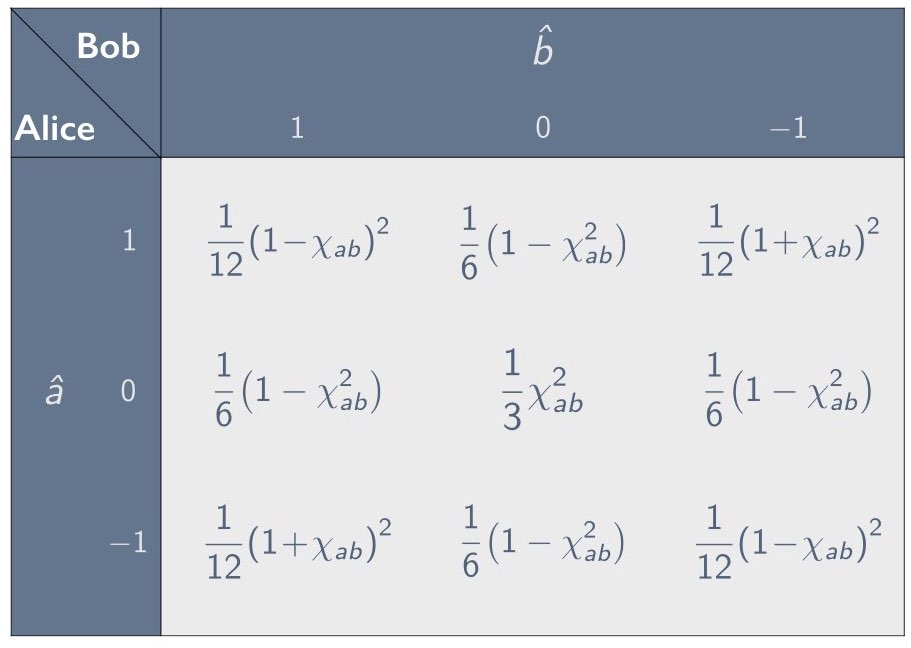
\includegraphics[width=4in]{CA-cell-spin1-chi.jpeg} 
   \caption{Cell in a correlation array given by quantum mechanics for measurements on the singlet state of two spin-1 particles ($\chi_{ab} = \cos{\varphi_{ab}}$).}
    \label{CA-cell-spin1-chi}
\end{figure}

The $\hat{a} \, \hat{c}$ and $\hat{b} \, \hat{c}$ cells of the correlation arrays will have the exact same structure as $\hat{a} \, \hat{b}$ one, with $\varphi_{ab}$ replaced by $\varphi_{ac}$ and $\varphi_{bc}$. The correlation arrays for measurements on the singlet state of two spin-$\frac12$ or two spin-1 particles can thus be parametrized by the cosines of the angles $\varphi_{ab}$, $\varphi_{ac}$ and $\varphi_{bc}$ between the directions $\vec{e}_a$, $\vec{e}_b$ and $\vec{e}_c$ in which the spin is being measured. This is also true for the singlet state of two particles with higher spin \citep[Vol.\ 2, p.\ 1072, Eq.\ (3.72)]{Messiah 1962}. In Section \ref{2.1.5}, we will show that these cosines can be interpreted as anti-correlation coefficients, thereby justifying the notation introduced in Eq.\ (\ref{spin-s cosines}). 

  
%SUBSUBSECTION 3.1.4
\subsubsection{Non-signaling in the spin-$s$ case} \label{2.1.4}
%Showing that the correlations found in measurements on two particles with spin $s$ in the singlet state are non-signaling}

We now show that the correlations found in measurements on the singlet state of two particles of any (half-)integer spin $s$ have uniform marginals and are therefore non-signaling. Consider the correlation array in Figure \ref{CA-cell-spin1-chi} and the marginal probability of Alice finding the outcome $m_1 = 1$ when she uses setting $\hat{a}$ and Bob uses setting $\hat{b}$:
\begin{eqnarray} 
\mathrm{Pr}(+1_A| \hat{a}\, \hat{b}) \nonumber
& \!\!\! = \!\!\! &\sum_{m_2=-1}^1 \mathrm{Pr}(+1\,m_2| \hat{a}\, \hat{b}) \nonumber \\[.3 cm]
&\!\!\! = \!\!\!  &\; \frac{1}{12}(1+ \chi_{ab})^2+\frac{1}{6}(1- \chi_{ab}^2)+\frac{1}{12}(1- \chi_{ab})^2 = \frac13.
\label{nonsignal 1}
\end{eqnarray}
For $m_1=0$ and $m_1 = -1$ we similarly find that 
\begin{equation}
\mathrm{Pr}(0_A| \hat{a}\, \hat{b})=\mathrm{Pr}(-1_A| \hat{a}\, \hat{b})= \frac13.
\end{equation}
None of these marginal probabilities---and this observation is key---depend on $\varphi_{ab}$. They are thus unaltered if Bob's settings are changed from $\hat{b}$ to $\hat{a}$ or $\hat{c}$. The same is true for the marginal probabilities of Bob measuring $m_2 = (1, 0, -1)$ using any of these three settings. In every cell of the correlation array that the cell in  Figure \ref{CA-cell-spin1-chi} is part of, all three rows and all three columns add up to $\sfrac13$. Like the singlet state for a pair of spin-$\frac12$ particles, the singlet state for a pair of spin-1 particles thus cannot be used for superluminal signaling.

The same is true for the singlet state of two particles of higher spin. The marginal probability of Alice finding $m_1$ for $\hat{a}$ when Bob uses $\hat{b}$ is:
\begin{equation}
\mathrm{Pr}(m_{1}| \hat{a}\, \hat{b}) = \sum_{m_2=-s}^s \mathrm{Pr}(m_1 \,m_2| \hat{a}\, \hat{b}).
\end{equation}
Using the first line of Eq.\ (\ref{inner product 2}), we find that
\begin{eqnarray} 
\mathrm{Pr}(m_{1}| \hat{a}\, \hat{b}) 
& \!\!\! = \!\!\! &\frac{1}{2s+1} \! \sum_{m_2=-s}^s \! \Big|{_{2b}}\langle s, m_2|s, -m_1\rangle{_{2a}}\Big|^2 \label{nonsignal 2} \nonumber \\[.3 cm]
& \!\!\! = \!\!\! &\frac{1}{2s+1} \! \sum_{m_2=-s}^s \!
{_{2a}}\langle s, -m_1|s,m_2\rangle{_{2b}}\; {_{2b}}\langle s, m_2|s,-m_1\rangle{_{2a}}.
\end{eqnarray}
Evaluating this sum, using the completeness relation
\begin{equation}
\hat{1}_2 = \sum_{m=-s}^s |s,m \rangle_{\!2b}\; {_{2b\!}}\langle s, m|,
\label{completeness}
\end{equation}
%i.e., the resolution of unity in the orthonormal basis $\{|s,m \rangle_{2b}\}_{m=-s}^s$ 
%(see Eq.\ (\ref{onb one-particle Hilbert space})) 
%for the second particle,
we arrive at
\begin{equation}
\mathrm{Pr}(m_{1}| \hat{a}\, \hat{b}) = \frac{1}{2s+1} \;
{_{2a}}\langle s, -m_1|s,-m_1\rangle{_{2a}} = \frac{1}{2s+1}.
\label{nonsignal 3}
\end{equation}
This same formula holds if we substitute $m_2$ for $m_1$ or any two of the triplet of settings $(\hat{a}, \hat{b}, \hat{c})$ for $\hat{a}\, \hat{b}$. It follows that the correlations found in the measurements on the singlet state of two spin-$s$ particles are indeed non-signaling. In every cell of the corresponding correlation array, all $2s+1$ rows and all $2s+1$ columns sum to $1/(2s+1)$.   

%SUBSUBSECTION 3.1.5
\subsubsection{Anti-correlation coefficients in the spin-$s$ case} \label{2.1.5}

We now turn our attention to the quantities $\chi_{ab}$ introduced in Eq.\ (\ref{spin-s cosines}) and the analogous quantities $\chi_{ac}$ and $\chi_{bc}$. We show that these can be interpreted as anti-correlation coefficients just as in the case of $s = \sfrac12$ (see Eqs.\ (\ref{chi values repeat})--(\ref{chi2angle}) in Section \ref{1.5}). Consider the expectation value
\begin{equation}
\langle \hat{S}_{1a}\hat{S}_{2b}\rangle_{00}\equiv {_{12\!}}\langle 0,0|\hat{S}_{1a}\hat{S}_{2b}|0,0\rangle_{12}.
\label{exp def}
\end{equation}
Recalling our choice of $\vec{e}_a$ and $\vec{e}_b$ in Eq.\ (\ref{vector dirs 2}), we have
\begin{equation}
\hat{S}_{1a} = \hat{S}_{1z}, \quad \hat{S}_{2b} = \hat{S}_{2z}  \cos{\varphi_{ab}} + \hat{S}_{2x}  \sin{\varphi_{ab}}. 
\label{rewriting Sa and Sb}
\end{equation}
Inserting these expressions into Eq.\ (\ref{exp def}), we arrive at:
\begin{equation}
\langle \hat{S}_{1a}\hat{S}_{2b}\rangle_{00} = \langle \hat{S}_{1z}\hat{S}_{2z}\rangle_{00} \cos\varphi_{ab}+\langle \hat{S}_{1z}\hat{S}_{2x}\rangle_{00} \sin \varphi_{ab}.
\label{exp value 1}
\end{equation}
The quantity $\langle \hat{S}_{1z}\hat{S}_{2z}\rangle_{00}$ in the first term on the right-hand side is minus the square of the standard deviation $\sigma_s$ (see Eq.\ (\ref{SD for adm raffle 1}) in Section \ref{1.6}). This quantity is thus given by
\begin{equation}
\langle \hat{S}_{1z}\hat{S}_{2z}\rangle_{00} = \sigma_s^2 = - \frac13 s(s+1).
\label{SD for singlet state}
\end{equation}
This same result can be derived directly from properties of the singlet state. The expectation value of the product of $\hat{S}_{1z}$ and $\hat{S}_{2z}$ in the singlet state is given by
\begin{equation}
\langle \hat{S}_{1z} \hat{S}_{2z} \rangle_{00}  = {_{12\!}}\langle 0,0| \hat{S}_{1z}\hat{S}_{2z}|0,0\rangle_{\!12}.
\label{aa product prob 1}  
\end{equation}
Using that $\hat{S}_{2z} = \hat{S}_z - \hat{S}_{1z}$ and that $\hat{S}_z  |0,0\rangle_{\!12} = 0$, we can rewrite this as
\begin{equation}
\langle \hat{S}_{1z} \hat{S}_{2z} \rangle_{00} = -{_{12\!}}\langle 0,0| \hat{S}_{1z}^2|0,0\rangle_{12}.
\label{aa product prob 2} 
\end{equation}
Rotational invariance requires that 
\begin{equation}
{_{12\!}}\langle 0,0| \hat{S}_{1x}^2|0,0\rangle_{12} = {_{12\!}}\langle 0,0| \hat{S}_{1y}^2|0,0\rangle_{12} = {_{12\!}}\langle 0,0| \hat{S}_{1z}^2|0,0\rangle_{12}.
\label{aa product prob 3}  
\end{equation}
Hence
\begin{equation}
\langle \hat{S}_{1z} \hat{S}_{2z} \rangle_{00} = - \frac13 \, {_{12\!}}\langle 0,0| \big( \hat{S}_{1x}^2+\hat{S}_{1y}^2+\hat{S}_{1z}^2 \big) |0,0\rangle_{\!12}.
\label{aa product prob 4}  
\end{equation}
Substituting $\hat{S}_{1}^2$ for $\hat{S}_{1x}^2+\hat{S}_{1y}^2+\hat{S}_{1z}^2$ and using that $\hat{S}_{1}^2 |0,0\rangle_{\!12} = s(s+1) |0,0\rangle_{12}$, we recover Eq.\ (\ref{SD for singlet state}): 
\begin{equation}
\langle \hat{S}_{1z} \hat{S}_{2z} \rangle_{00} = -\frac13 \, {_{12\!}}\langle 0,0| \hat{S}_{1}^2|0,0\rangle_{\!12}  = -\frac13 s(s+1).
\label{aa product prob 5} 
\end{equation}
 
Again using the rotational invariance of the singlet state, we can show that the second term in Eq.\ (\ref{exp value 1}) vanishes. Consider a rotation of the singlet state over $180\degree$ around the $z$-axis. Since the singlet state is invariant under arbitrary rotation, the action of the operator $e^{-i\pi \hat{S}_z}$ implementing this rotation (see Eq.\ (\ref{ops rot})) on the singlet state simply reproduces the singlet state. It follows that
\begin{equation}
\langle \hat{S}_{1z}\hat{S}_{2x}\rangle_{00} = {_{12\!}}\langle 0,0| \hat{S}_{1z}\hat{S}_{2x}|0,0\rangle_{\!12} =  {_{12\!}}\langle 0,0|e^{i\pi \hat{S}_z} \hat{S}_{1z}\hat{S}_{2x}e^{-i\pi \hat{S}_z}|0,0\rangle_{\!12}.
\label{exp value 2 a}
\end{equation}
Inserting $\hat{S}_z = \hat{S}_{1z} + \hat{S}_{2z}$ and using that $\hat{S}_{1z}$ commutes with both $\hat{S}_{2z}$ and $\hat{S}_{2x}$, we can rewrite this as:
\begin{equation}
\langle \hat{S}_{1z}\hat{S}_{2x}\rangle_{00} = {_{12\!}}\langle 0,0| \hat{S}_{1z} \, e^{i\pi \hat{S}_{2z}}\hat{S}_{2x}e^{-i\pi \hat{S}_{2z}} |0,0\rangle_{\!12}.
\label{exp value 2 b}
\end{equation}
Recalling the transformation law for spin operators in Eq.\ (\ref{ops rot}), we note that:
\begin{equation}
\quad e^{i\pi \hat{S}_{2z}}\hat{S}_{2x}e^{-i\pi \hat{S}_{2z}} = -\hat{S}_{2x}.
\label{exp value 2 c}
\end{equation}
Inserting this expression into Eq.\ (\ref{exp value 2 b}), we conclude that
\begin{equation}
\langle \hat{S}_{1z}\hat{S}_{2x}\rangle_{00} = - {_{12\!}}\langle 0,0|  \hat{S}_{1z}\hat{S}_{2x} |0,0\rangle_{\!12} =  - \langle \hat{S}_{1z}\hat{S}_{2x} \rangle_{00} = 0.
\label{exp value 2 d}
\end{equation}
So the only contribution to Eq.\ (\ref{exp value 1}) comes from the first term: 
\begin{equation}
\langle \hat{S}_{1a}\hat{S}_{2b}\rangle_{00} = \langle \hat{S}_{1a}\hat{S}_{2a} \rangle_{00} \cos\varphi_{ab} = -\frac13 s(s+1) \, \chi_{ab},
\label{exp value 3}
\end{equation} 
where we used Eq.\  (\ref{aa product prob 5})) for $ \langle \hat{S}_{1a}\hat{S}_{2a} \rangle_{00}$ and the definition of $\chi_{ab}$ in Eq.\ (\ref{spin-s cosines}). Using that the standard deviations 
\begin{equation}
\sigma_{1a} \equiv \sqrt{\langle \hat{S}_{1a}^2 \rangle_{00} } \quad {\mathrm{and}} \quad
\sigma_{2b} \equiv \sqrt{ \langle \hat{S}_{2b}^2 \rangle_{00} }
\label{sigma s > 1/2 a} 
\end{equation}
are both given by Eq.\ (\ref{SD for singlet state}), we can rewrite Eq.\ (\ref{exp value 3}) as
\begin{equation}
\chi_{ab} = - \frac{\langle \hat{S}_{1a}\hat{S}_{2b}\rangle_{00}}{\sigma_a \sigma_b}
\end{equation}
which we recognize as the definition of the anti-correlation coefficient $\chi_{ab}$ (see Section \ref{1.3}, Eq.\ (\ref{chi as corr coef}), and Section \ref{1.5}, Eq.\ (\ref{chi2angle})). This justifies the use of the $\chi_{ab}$ notation in Eq.\ (\ref{spin-s cosines}). This identification moreover means that the main conclusion of our examination of the special case of spin-$\frac12$ particles in Section \ref{1.5} carries over to the general case considered in this section: the set of values for $(\chi_{ab},\chi_{ac},\chi_{bc})$ that can be obtained by measurements on the singlet state of two particles of higher spin is the elliptope in Figure \ref{elliptope}.

%SUBSUBSECTION 3.1.6
\subsubsection{Cell symmetries in the spin-$s$ case} \label{2.1.6}

In this subsection, we will consider various symmetries of cells in correlation arrays for measurements on particles of arbitrary (half-)integer spin $s$.  Figures \ref{CA-3set2out-non-signaling-halfangles} and \ref{CA-cell-spin1-chi} show such cells for the $s = \sfrac12$ and $s = 1$ cases. Figure \ref{CA-2set4out} shows it for the $s = \sfrac32$ case.

\begin{figure}[ht]
 \centering
   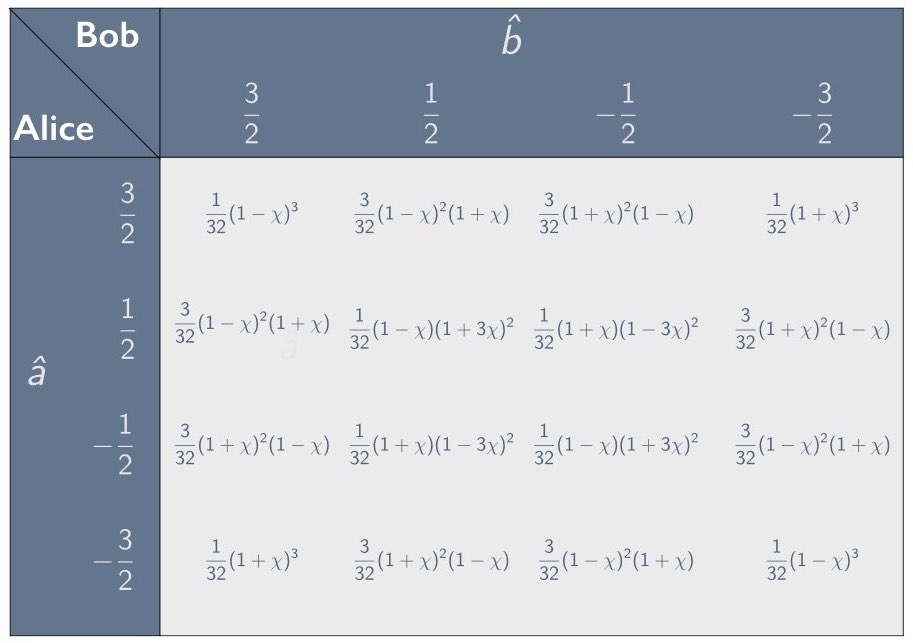
\includegraphics[width=4.5in]{CA-2set4out.jpeg} 
   \caption{Cell in a correlation array given by quantum mechanics for measurements on the singlet state of two spin-$\frac32$ particles ($\chi = \cos{\varphi_{ab}}$).}
   \label{CA-2set4out}
\end{figure} 

Cells on the diagonals in all these cases are particularly simple. Since for those cells $\chi_{ab} = \cos{\varphi_{ab}} =1$, elements on the skew-diagonal are equal and sum to 1 while the other elements are 0. This is true not just for  $s = \sfrac12$ and $s = 1$, but for any (half-)integer value of $s$. Whenever the angle between the measuring directions used by Alice and Bob is zero,  Eq.\ (\ref{wigner}) for the Wigner d-matrix element reduces to   
\begin{equation}
d^{\,(s)}_{-m_1m_2}(0) = {_z} \langle s, -m_1  | s, m_2 \rangle_z=\delta_{-m_1m_2}.
\label{wigner zero}
\end{equation}
Hence, the probability for Alice to measure $m_1$ and Bob to measure $m_2$ along a common direction, say $\vec{e}_a$, is given by (cf.\ Eq.\ (\ref{prob 3})):
\begin{equation}
\mathrm{Pr}(m_1\, m_2 | \hat{a}\,\hat{a} ) = \frac{1}{2s+1} \Big( \, d^{\,(s)}_{-m_1m_2}(0) \, \Big)^{2\!}=\frac{1}{2s+1} \, \delta_{-m_1m_2}.
\label{prob 4}
\end{equation}
Any cell on the diagonal of a correlation array for measurements on the singlet state of two particles of any integer or half-integer spin $s$  thus has values $1/(2s+1)$ on the skew-diagonal and zeros everywhere else (see Figure \ref{diag-cell-sxs} in Section \ref{1.6}).  

The off-diagonal cells, while not as simple as the diagonal ones, also exhibit features that are the same for all values of $s$. Note, for instance, that the cells in Figure \ref{CA-3set2out-non-signaling-halfangles} (for $s = \sfrac12$) and Figures \ref{CA-cell-spin1-chi}--\ref{CA-2set4out} (for $s = 1$ and $s = \sfrac32$) are all symmetric across both the diagonal and the skew-diagonal. This is true not just for $s = \sfrac12$ and $s = 1$ but for any (half-)integer $s$. This follows directly from the following three symmetry properties of the Wigner d-matrix in Eq.\ (\ref{wigner}):
%, i.e., from symmetries of the matrix elements for the one-particle rotation operator $e^{-i\vartheta \hat{S}_y}$:
\begin{eqnarray}
d^{\,(s)}_{mm'}(\vartheta) 
&\!\!=\!\!& (-1)^{m-m'} d^{\,(s)}_{m' m}(\vartheta) \label{WignerD sym 1} \quad \\[.3 cm] 
&\!\!=\!\!& (-1)^{m-m'} d^{\,(s)}_{-m-m'}(\vartheta) \label{WignerD sym 2} \\[.3 cm]
&\!\!=\!\!& d^{\,(s)}_{-m'-m}(\vartheta). \label{WignerD sym 3}
\end{eqnarray}

To establish the first of these symmetries, consider a rotation of the one-particle system through an angle of $180\degree$ around the $z$-axis, implemented as $e^{-i \pi \hat{S}_z}$. Such a rotation leaves the $z$-axis unchanged and as such the states are only changed up to an overall phase factor, i.e.,
\begin{equation}
    e^{-i\pi \hat{S}_z}| s, m \rangle_{z} = e^{-i \pi m}| s, m \rangle_{z}. 
    \label{WignerD sym 1 proof a}
\end{equation}
By contrast, this rotation flips the $y$-axis, which means that the operator $\hat{S}_y$ transforms as
\begin{equation}
    e^{-i\pi \hat{S}_z} \hat{S}_y e^{i\pi \hat{S}_z} = -\hat{S}_y.
\end{equation}
The same is true for any function of $\hat{S}_y$:
\begin{equation}
 e^{-i\pi \hat{S}_z} f(\hat{S}_y) \, e^{i\pi \hat{S}_z} = f(-\hat{S}_y).
\end{equation}
Hence, we can rewrite the Wigner d-matrix element in Eq.\ (\ref{wigner}) as
\begin{equation}
 d^{\,(s)}_{mm'}(\vartheta) = {_{z\!}}\langle s, m |e^{-i \vartheta \hat{S}_{y}}| s, m' \rangle_{z} = {_{z\!}}\langle s, m |e^{-i\pi \hat{S}_z}e^{i \vartheta \hat{S}_{y}}e^{i\pi \hat{S}_z}| s, m' \rangle_{z}.
\end{equation}
On account of Eq.\ (\ref{WignerD sym 1 proof a}), this reduces to: 
\begin{equation}
 d^{\,(s)}_{mm'}(\vartheta) = {_{z\!}}\langle s, m |e^{-i\pi m}e^{i \vartheta \hat{S}_{y}}e^{i\pi m'}| s, m' \rangle_{z} = (-1)^{m-m'} d^{\,(s)}_{mm'}(-\vartheta).
  \label{symm of W d-matrices 1}
\end{equation}
%As we noted in the discussion of raising and lowering operators, 
Given the Condon-Shortley phase convention, the operator $i\hat{S}_y$ has real matrix elements in the $|s,m\rangle_{\!z}$ basis (see Eqs.\ (\ref{raising operator})--(\ref{coef raising})). Since the elements of the Wigner d-matrix are matrix elements of a function of $i\hat{S}_y$  in this basis, it follows that they too must be real.
We can thus rewrite $d^{\,(s)}_{mm'}(-\vartheta)$ in Eq.\ (\ref{symm of W d-matrices 1}) as:
\begin{eqnarray}
    d^{\,(s)}_{mm'}(-\vartheta) 
    &\!\!=\!\!& d^{\,(s)}_{mm'}(-\vartheta) ^* \nonumber\\[.3 cm]
    &\!\!=\!\!& {_{z\!}}\langle s, m |e^{i \vartheta \hat{S}_{y}}| s, m' \rangle_{z}^* \nonumber\\[.3 cm]
    &\!\!=\!\!& {_{z\!}}\langle s, m' |e^{-i \vartheta \hat{S}_{y}}| s, m \rangle_{z} \nonumber \\[.3 cm]
    &\!\!=\!\!& d^{\,(s)}_{m'm}(\vartheta).
    \label{symm of W d-matrices 2}
\end{eqnarray}
Inserting this expression in Eq.\ (\ref{symm of W d-matrices 1}), we arrive at the symmetry stated in Eq.\ (\ref{WignerD sym 1}). 

To establish the second symmetry of the Wigner d-matrix, the one in Eq.\ (\ref{WignerD sym 2}), we consider a rotation through an angle of $180\degree$ around the $y$-axis, as implemented by $e^{-i\pi \hat{S}_y}$. This leaves $\hat{S}_y$ unchanged but flips $\hat{S}_z$. Thus the action of this rotation operator on the state $|s,m\rangle_z$---aside from on overall phase factor\footnote{This phase factor appears in \citet[Vol.\ 2, p.\ 1071, Eq.\ C65]{Messiah 1962} and may be proven for instance by appeal to Wigner's explicit formula (see p.\ 1072, Eq.\ C72 in Messiah) for the d-matrix elements. However, this phase factor does not enter into the probabilities and so we do not derive its value here.}
---is to replace $m$ by $-m$:
\begin{equation}
    e^{-i\pi \hat{S}_y} |s,m\rangle_z = (-1)^{s-m}|s,-m\rangle_z.
    \label{WignerD sym 2 proof a}
\end{equation}
Inserting the operators $e^{-i\pi \hat{S}_y}$ and $e^{i\pi \hat{S}_y}$ in the expression for the Wigner d-matrix in Eq.\ (\ref{wigner}),
\begin{equation}
 d^{\,(s)}_{mm'}(\vartheta) =  {_{z\!}}\langle s, m |e^{-i\pi \hat{S}_y}e^{-i \vartheta \hat{S}_{y}}e^{i\pi \hat{S}_y}| s, m' \rangle_{z},
\end{equation}
and using Eq.\ (\ref{WignerD sym 2 proof a}), we arrive at the symmetry in Eq.\ (\ref{WignerD sym 2}):  
\begin{eqnarray}
    d^{\,(s)}_{mm'}(\vartheta) &\!\!=\!\!& {_{z\!}}\langle s, -m |(-1)^{s-m}e^{-i \vartheta \hat{S}_{y}}(-1)^{s-m'}| s, -m' \rangle_{z} \nonumber \\[.3 cm]
    &\!\!=\!\!& (-1)^{m-m'} d^{\,(s)}_{-m-m'}(-\vartheta),
      \label{WignerD sym 2 proof b}
\end{eqnarray}
where in the last step we used that $(-1)^{s-m'}=(-1)^{m'-s}$.

The third symmetry of the Wigner d-matrix, the one in Eq.\ (\ref{WignerD sym 3}), follows as a corollary of the first two, the ones in Eqs.\ (\ref{WignerD sym 1}) and (\ref{WignerD sym 2}), though it can also be established directly through an argument similar to those in Eqs.\ (\ref{WignerD sym 1 proof a})--(\ref{symm of W d-matrices 2}) and Eqs.\ (\ref{WignerD sym 2 proof a})--(\ref{WignerD sym 2 proof a}), involving a rotation around the $x$-axis. 

These three symmetries of the Wigner d-matrix translate into three symmetries of the probabilities in Eq.\ (\ref{prob 3}):
\begin{equation}
\begin{array}{lcll}
\mathrm{Pr}(m_1 \, m_2 | \hat{a}\,\hat{b} ) & \!\!\! =  \!\!\! & \mathrm{Pr}(-m_2  -\!m_1 | \hat{a}\,\hat{b}) & \quad \quad {\mathrm{persymmetry}} \\[.3 cm]
  & \!\!\! =  \!\!\! & \mathrm{Pr}(-m_1  -\!m_2 | \hat{a}\,\hat{b}) & \quad \quad {\mathrm{centrosymmetry}}  \\[.3 cm]
  & \!\!\! =  \!\!\! & \mathrm{Pr}(m_2 \, m_1 | \hat{a}\,\hat{b} ) & \quad \quad {\mathrm{symmetry}}.    
\end{array}
\label{Prob sym}
\end{equation}
This tells us that the probability is unchanged if we either swap $m_1$ and $m_2$ or flip both of their signs. These symmetries, in turn, translate into symmetries of any cell in a correlation array for measurements on the singlet state of two particles with spin $s$. The first line in Eq.\ (\ref{Prob sym}) expresses that any such cell is \emph{persymmetric}, i.e., symmetric across its main anti-diagonal; the second that it is \emph{centrosymmetric}, i.e., symmetric about its center; the third that it is \emph{symmetric}, i.e., symmetric across its main diagonal. Any two of these symmetries imply the third. As we noted in the introduction to Section \ref{2}, in the spin-$\frac12$ case, centrosymmetry implies both symmetry and persymmetry. Since the design of our raffle tickets guarantees centrosymmetry, we did not have to impose any conditions on our raffles to ensure all three symmetries. As we will see in Section \ref{2.2}, however, such conditions are needed for higher-spin cases if we want our raffles to give correlation arrays with the same symmetries as the quantum correlation arrays they are supposed to simulate. 
